% ----------------------------------------------
% ARCHITECTURE MATERIELLE ET LOGICIELLE {p.TODO}
% ----------------------------------------------
\subsubsection{Architecture matérielle et logicielle}
Le diagramme de déploiement UML de la figure \ref{schema_arch_mat} du projet représente l'architecture matérielle et logicielle du SàE. Les conventions graphiques utilisées sont explicitées sur la figure \ref{schema_legende_diag_deploiment}. Ce diagramme de déploiement identifie les entités matérielles et/ou logicielles avec lesquelles le SàE doit intéragir et permet ainsi de déterminer les principaux échanges qu'il entretient avec son environnement. 
\begin{figure}[ht] 
    \centering
    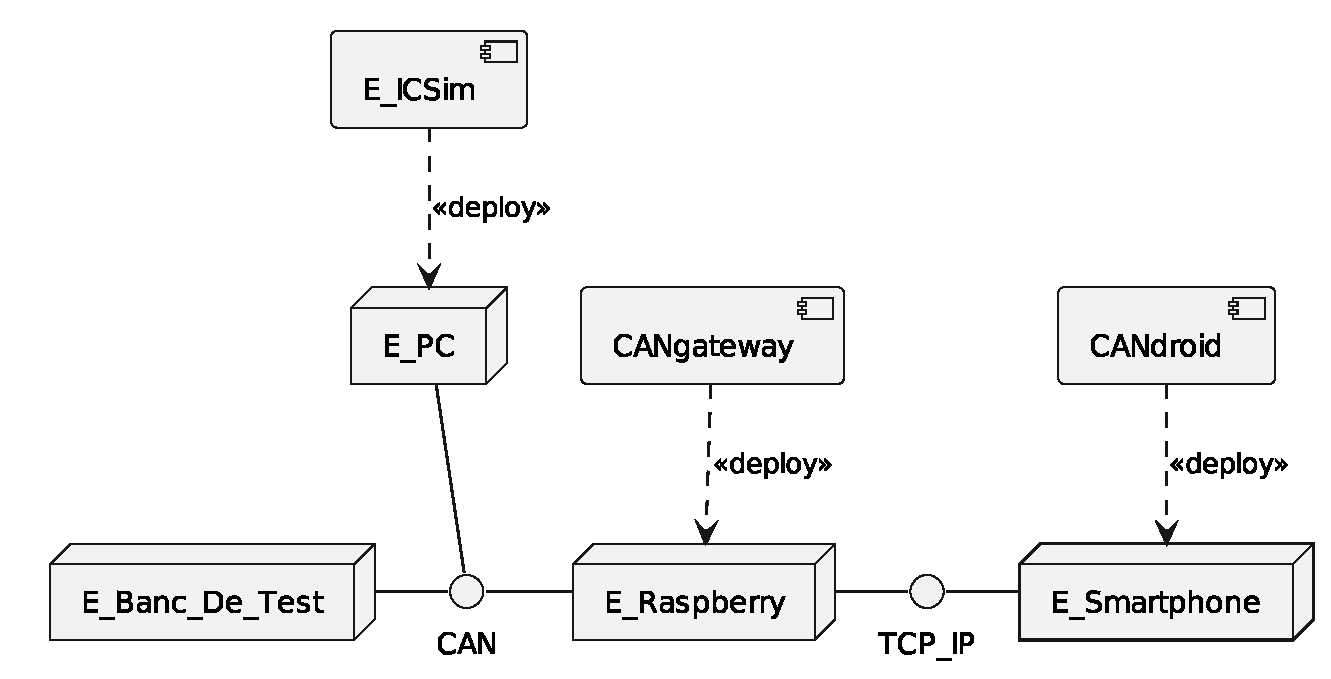
\includegraphics[width=14cm]{../schemas/arch_mat}
    \captionsetup{justification=centering}
    \caption{Architecture matérielle et logicielle représentée \\par un diagramme de déploiement UML}
    \label{schema_arch_mat}
\end{figure}

Comme indiqué sur le diagramme, l'application {\nomApplication} est déployée sur E\_Smartphone. Le programme {\nomLogiciel} est déployé sur E\_Raspberry. E\_Smartphone et E\_Raspberry communiquent ensemble grâce au protocole \hyperref[tcp_ip]{TCP/IP}. E\_Raspberry récupère les trames CAN émisent par E\_PC et/ou E\_Banc\_De\_Test grâce au RS485 CAN Hat qui permet à E\_Raspberry d'utiliser le protocole de communication CAN (Voir section \ref{dictionnaire}). E\_ICSim est un logiciel de simulation déployé sur E\_PC. Il permettra aux futurs utilisateurs de se former aux protocoles de communication CAN sans avoir à utiliser un Banc de test encombrant. Par convention, le nom de ces entités est préfixé par les caractères {\guillemotleft} E\_ {\guillemotright} (E pour Extern). Les caractéristiques de ces entités sont décrites dans le dictionnaire du domaine (voir section \ref{dictionnaire}).
\begin{figure}[ht] 
    \centering
    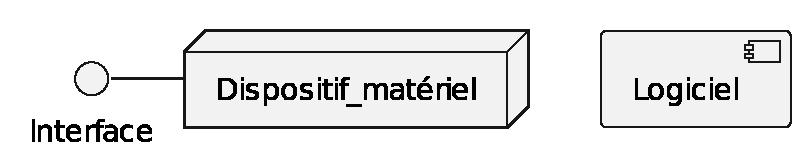
\includegraphics[width=10cm]{../schemas/legende_diag_deploiement}
    \caption{Légende du diagramme de déploiement UML}
    \label{schema_legende_diag_deploiment}
\end{figure}

\bigskip